%%%%%%%%%%%%%%%%%%%%%%%%%%%%%%%%%%%%%%%%%
% Programming/Coding Assignment
% LaTeX Template
%
% This template has been downloaded from:
% http://www.latextemplates.com
%
% Original author:
% Ted Pavlic (http://www.tedpavlic.com)
%
% Note:
% The \lipsum[#] commands throughout this template generate dummy text
% to fill the template out. These commands should all be removed when 
% writing assignment content.
%
% This template uses a Perl script as an example snippet of code, most other
% languages are also usable. Configure them in the "CODE INCLUSION 
% CONFIGURATION" section.
%
%%%%%%%%%%%%%%%%%%%%%%%%%%%%%%%%%%%%%%%%%

%----------------------------------------------------------------------------------------
%	PACKAGES AND OTHER DOCUMENT CONFIGURATIONS
%----------------------------------------------------------------------------------------

\documentclass{article}

\usepackage{fancyhdr} % Required for custom headers
\usepackage{lastpage} % Required to determine the last page for the footer
\usepackage{extramarks} % Required for headers and footers
\usepackage[usenames,dvipsnames]{color} % Required for custom colors
\usepackage{graphicx} % Required to insert images
\usepackage{listings} % Required for insertion of code
\usepackage{courier} % Required for the courier font
\usepackage{lipsum} % Used for inserting dummy 'Lorem ipsum' text into the template
\usepackage{hyperref}

% Margins
\topmargin=-0.45in
\evensidemargin=0in
\oddsidemargin=0in
\textwidth=6.5in
\textheight=9.0in
\headsep=0.25in

\linespread{1.1} % Line spacing

% Set up the header and footer
\pagestyle{fancy}
\lhead{\hmwkAuthorName} % Top left header
\chead{\hmwkClass\ (\hmwkClassInstructor\ \hmwkClassTime): \hmwkTitle} % Top center head
\rhead{\firstxmark} % Top right header
\lfoot{\lastxmark} % Bottom left footer
\cfoot{} % Bottom center footer
\rfoot{Page\ \thepage\ of\ \protect\pageref{LastPage}} % Bottom right footer
\renewcommand\headrulewidth{0.4pt} % Size of the header rule
\renewcommand\footrulewidth{0.4pt} % Size of the footer rule

\setlength\parindent{0pt} % Removes all indentation from paragraphs

%----------------------------------------------------------------------------------------
%	CODE INCLUSION CONFIGURATION
%----------------------------------------------------------------------------------------

\definecolor{MyDarkGreen}{rgb}{0.0,0.4,0.0} % This is the color used for comments
\lstloadlanguages{Perl} % Load Perl syntax for listings, for a list of other languages supported see: ftp://ftp.tex.ac.uk/tex-archive/macros/latex/contrib/listings/listings.pdf
\lstset{language=Perl, % Use Perl in this example
        frame=single, % Single frame around code
        basicstyle=\small\ttfamily, % Use small true type font
        keywordstyle=[1]\color{Blue}\bf, % Perl functions bold and blue
        keywordstyle=[2]\color{Purple}, % Perl function arguments purple
        keywordstyle=[3]\color{Blue}\underbar, % Custom functions underlined and blue
        identifierstyle=, % Nothing special about identifiers                                         
        commentstyle=\usefont{T1}{pcr}{m}{sl}\color{MyDarkGreen}\small, % Comments small dark green courier font
        stringstyle=\color{Purple}, % Strings are purple
        showstringspaces=false, % Don't put marks in string spaces
        tabsize=5, % 5 spaces per tab
        %
        % Put standard Perl functions not included in the default language here
        morekeywords={rand},
        %
        % Put Perl function parameters here
        morekeywords=[2]{on, off, interp},
        %
        % Put user defined functions here
        morekeywords=[3]{test},
       	%
        morecomment=[l][\color{Blue}]{...}, % Line continuation (...) like blue comment
        numbers=left, % Line numbers on left
        firstnumber=1, % Line numbers start with line 1
        numberstyle=\tiny\color{Blue}, % Line numbers are blue and small
        stepnumber=5, % Line numbers go in steps of 5
        breaklines=true
}

% Creates a new command to include a perl script, the first parameter is the filename of the script (without .pl), the second parameter is the caption
\newcommand{\pythonscript}[2]{
\begin{itemize}
\item[]\lstinputlisting[caption=#2,label=#1]{#1.py}
\end{itemize}
}

%----------------------------------------------------------------------------------------
%	DOCUMENT STRUCTURE COMMANDS
%	Skip this unless you know what you're doing
%----------------------------------------------------------------------------------------

% Header and footer for when a page split occurs within a problem environment
\newcommand{\enterProblemHeader}[1]{
\nobreak\extramarks{#1}{#1 continued on next page\ldots}\nobreak
\nobreak\extramarks{#1 (continued)}{#1 continued on next page\ldots}\nobreak
}

% Header and footer for when a page split occurs between problem environments
\newcommand{\exitProblemHeader}[1]{
\nobreak\extramarks{#1 (continued)}{#1 continued on next page\ldots}\nobreak
\nobreak\extramarks{#1}{}\nobreak
}

\setcounter{secnumdepth}{0} % Removes default section numbers
\newcounter{homeworkProblemCounter} % Creates a counter to keep track of the number of problems

\newcommand{\homeworkProblemName}{}
\newenvironment{homeworkProblem}[1][Problem \arabic{homeworkProblemCounter}]{ % Makes a new environment called homeworkProblem which takes 1 argument (custom name) but the default is "Problem #"
\stepcounter{homeworkProblemCounter} % Increase counter for number of problems
\renewcommand{\homeworkProblemName}{#1} % Assign \homeworkProblemName the name of the problem
\section{\homeworkProblemName} % Make a section in the document with the custom problem count
\enterProblemHeader{\homeworkProblemName} % Header and footer within the environment
}{
\exitProblemHeader{\homeworkProblemName} % Header and footer after the environment
}

\newcommand{\problemAnswer}[1]{ % Defines the problem answer command with the content as the only argument
\noindent\framebox[\columnwidth][c]{\begin{minipage}{0.98\columnwidth}#1\end{minipage}} % Makes the box around the problem answer and puts the content inside
}

\newcommand{\homeworkSectionName}{}
\newenvironment{homeworkSection}[1]{ % New environment for sections within homework problems, takes 1 argument - the name of the section
\renewcommand{\homeworkSectionName}{#1} % Assign \homeworkSectionName to the name of the section from the environment argument
\subsection{\homeworkSectionName} % Make a subsection with the custom name of the subsection
\enterProblemHeader{\homeworkProblemName\ [\homeworkSectionName]} % Header and footer within the environment
}{
\enterProblemHeader{\homeworkProblemName} % Header and footer after the environment
}

%----------------------------------------------------------------------------------------
%	NAME AND CLASS SECTION
%----------------------------------------------------------------------------------------

\newcommand{\hmwkTitle}{Assignment\ \#2} % Assignment title
\newcommand{\hmwkDueDate}{Thursday,\ March\ 5,\ 2014} % Due date
\newcommand{\hmwkClass}{CS\ 851} % Course/class
\newcommand{\hmwkClassTime}{4:20pm} % Class/lecture time
\newcommand{\hmwkClassInstructor}{DR NELSON} % Teacher/lecturer
\newcommand{\hmwkAuthorName}{VICTOR NWALA} % Your name

%----------------------------------------------------------------------------------------
%	TITLE PAGE
%----------------------------------------------------------------------------------------

\title{
\vspace{2in}
\textmd{\textbf{\hmwkClass:\ \hmwkTitle}}\\
\normalsize\vspace{0.1in}\small{Due\ on\ \hmwkDueDate}\\
\vspace{0.1in}\large{\textit{\hmwkClassInstructor\ \hmwkClassTime}}
\vspace{3in}
}

\author{\textbf{\hmwkAuthorName}}
\date{} % Insert date here if you want it to appear below your name

%----------------------------------------------------------------------------------------

\begin{document}

\maketitle

%----------------------------------------------------------------------------------------
%	TABLE OF CONTENTS
%----------------------------------------------------------------------------------------

%\setcounter{tocdepth}{1} % Uncomment this line if you don't want subsections listed in the ToC

\newpage
\tableofcontents
\newpage

%----------------------------------------------------------------------------------------
%	PROBLEM 1
%----------------------------------------------------------------------------------------

% To have just one problem per page, simply put a \clearpage after each problem

\begin{homeworkProblem}
Choose 100 URIs from A1
\newline
Generate WARC files of those URIs using:
wget
WARCreate
Heritrix (stand-alone or via WAIL)
webrecorder.io
\newline
Describe the resulting WARC files: quantitatively compare \& contrast the results of the WARC files of the same URI as generated by different tools
choose interesting examples.
\newline
Demonstrate playback of 2-3 WARCs in the (Wayback Machine (via WAIL or stand-alone) or pywb) and (webrecorder.io)

\pythonscript{wgetWarc}{Script to download wget Warc files}




I used the same 103 URIs for wget, warcreate, webrecorder. I could not use the same 100 URIs for WAIL because of the delimeter errors I experience while doing it, so I changed the URI mixes to mininise the errors I experienced. I conbimed the warc file using WARCMerge.
\newline
In order to quantitatively compare the different methods, I selected 4 URIs to generate warc files using the 4 methods, and I discovered this:
Warcreate was over 33.5 MB, over because 1 URI failed to generate a warc file. WAIL was 3.71 MB, Web Recorder 4.6 MB, Wget 165.4 KB. Hence Warcreate warc files are the largest while wget warc files are the smallest.

\begin{center}
{Figure 1: Comparing file sizes for the different warc tools}
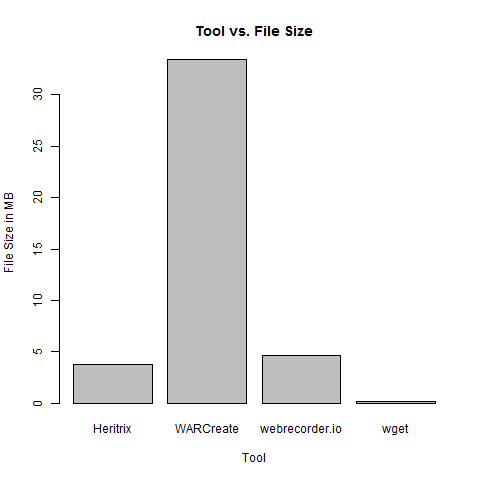
\includegraphics[width=0.75\columnwidth]{victor} 
\end{center}


\begin{center}
{Figure 2: Replaying Warc file with webrecorder}
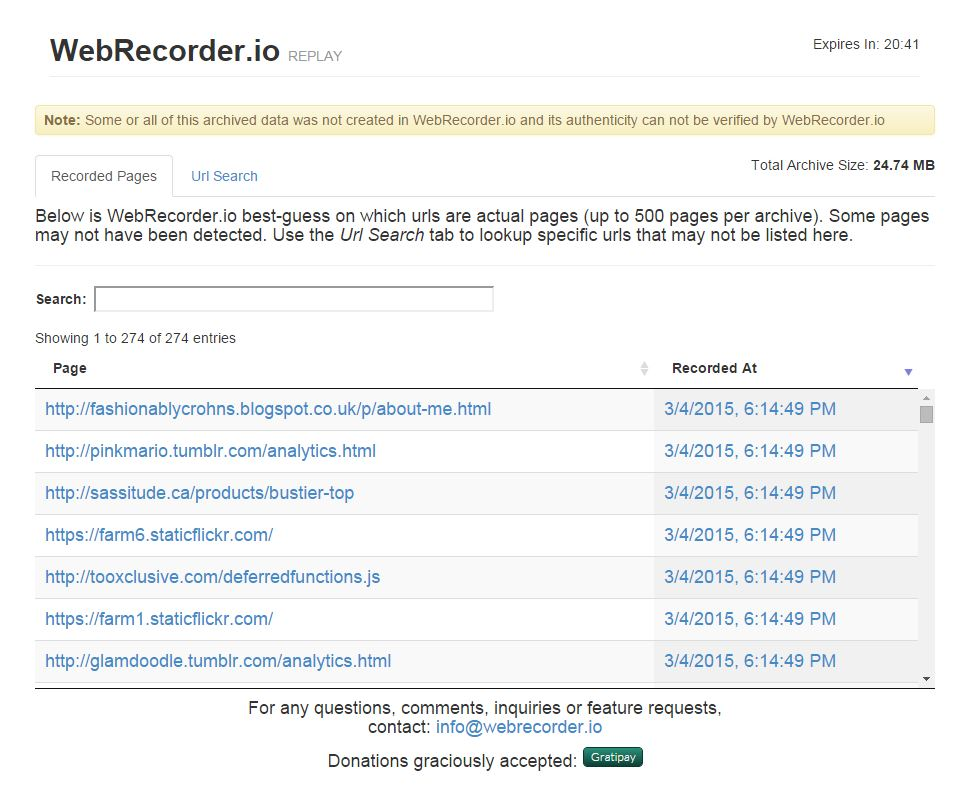
\includegraphics[width=0.75\columnwidth]{FirstWarcReplay} 
\end{center}

\begin{center}
{Figure 3: Replaying Warc file with webrecorder}
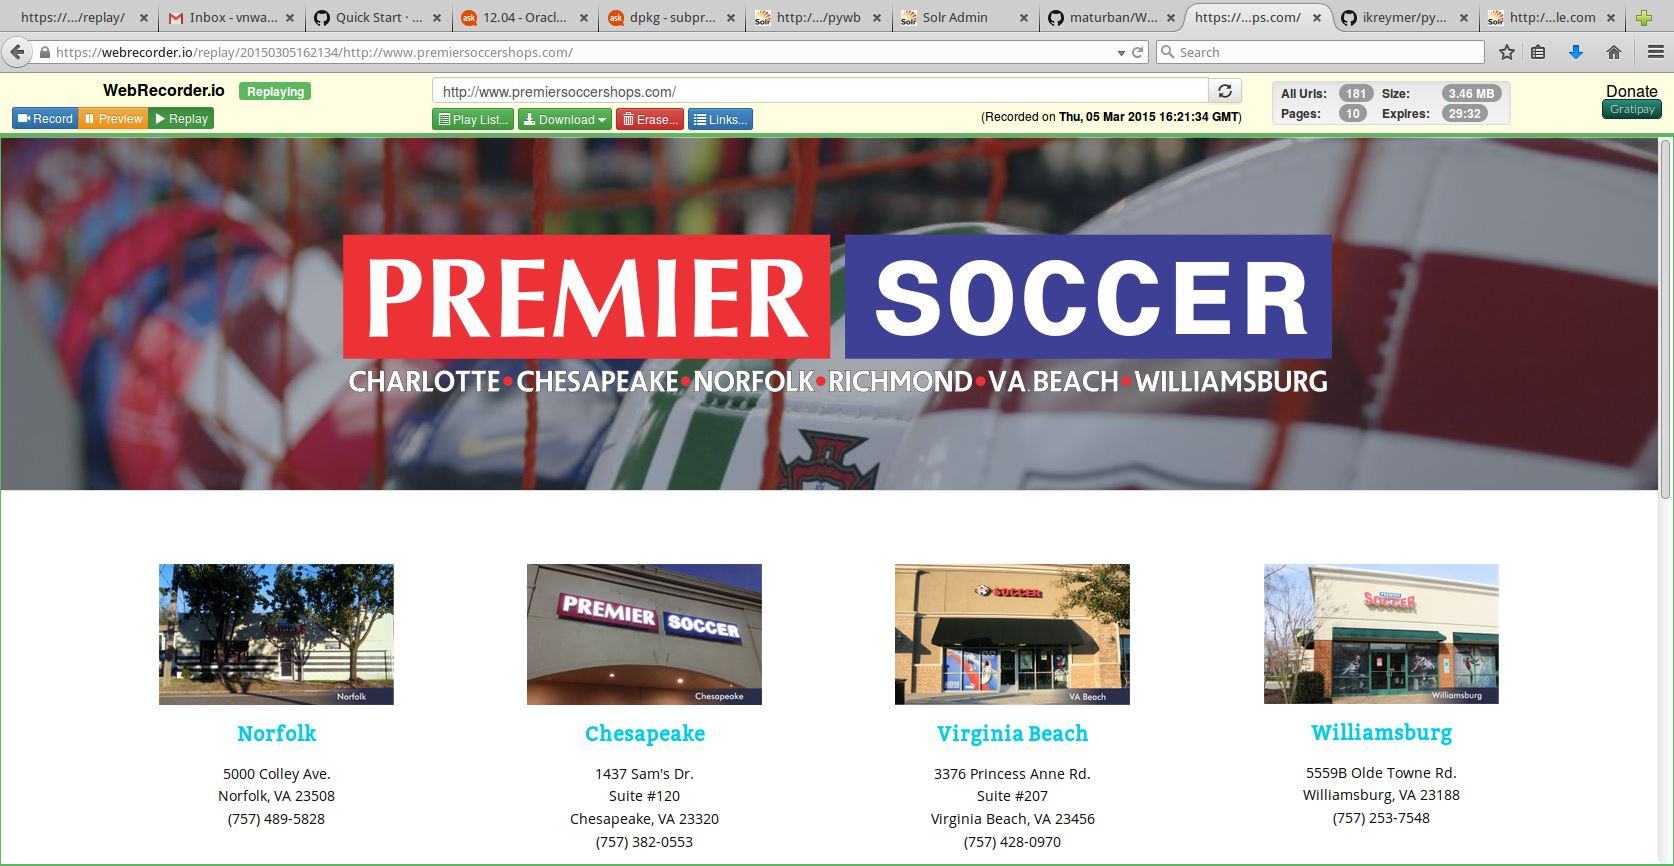
\includegraphics[width=0.75\columnwidth]{webRecorderReplay} 
\end{center}

\begin{center}
{Figure 4: Replaying Warc file with Wayback Machine}
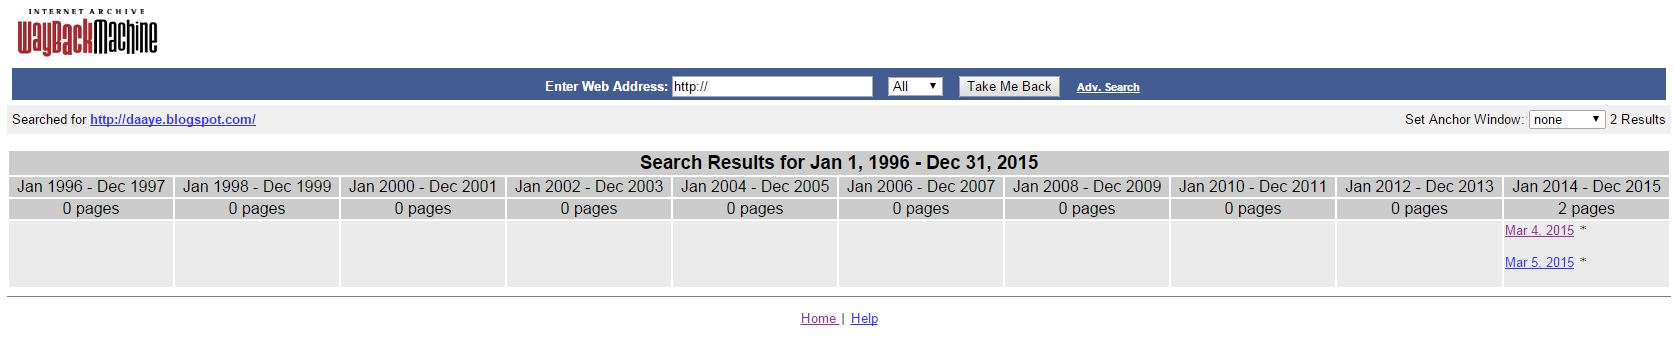
\includegraphics[width=0.75\columnwidth]{wayback} 
\end{center}


\begin{center}
{Figure 5: Replaying Warc file with Wayback Machine}
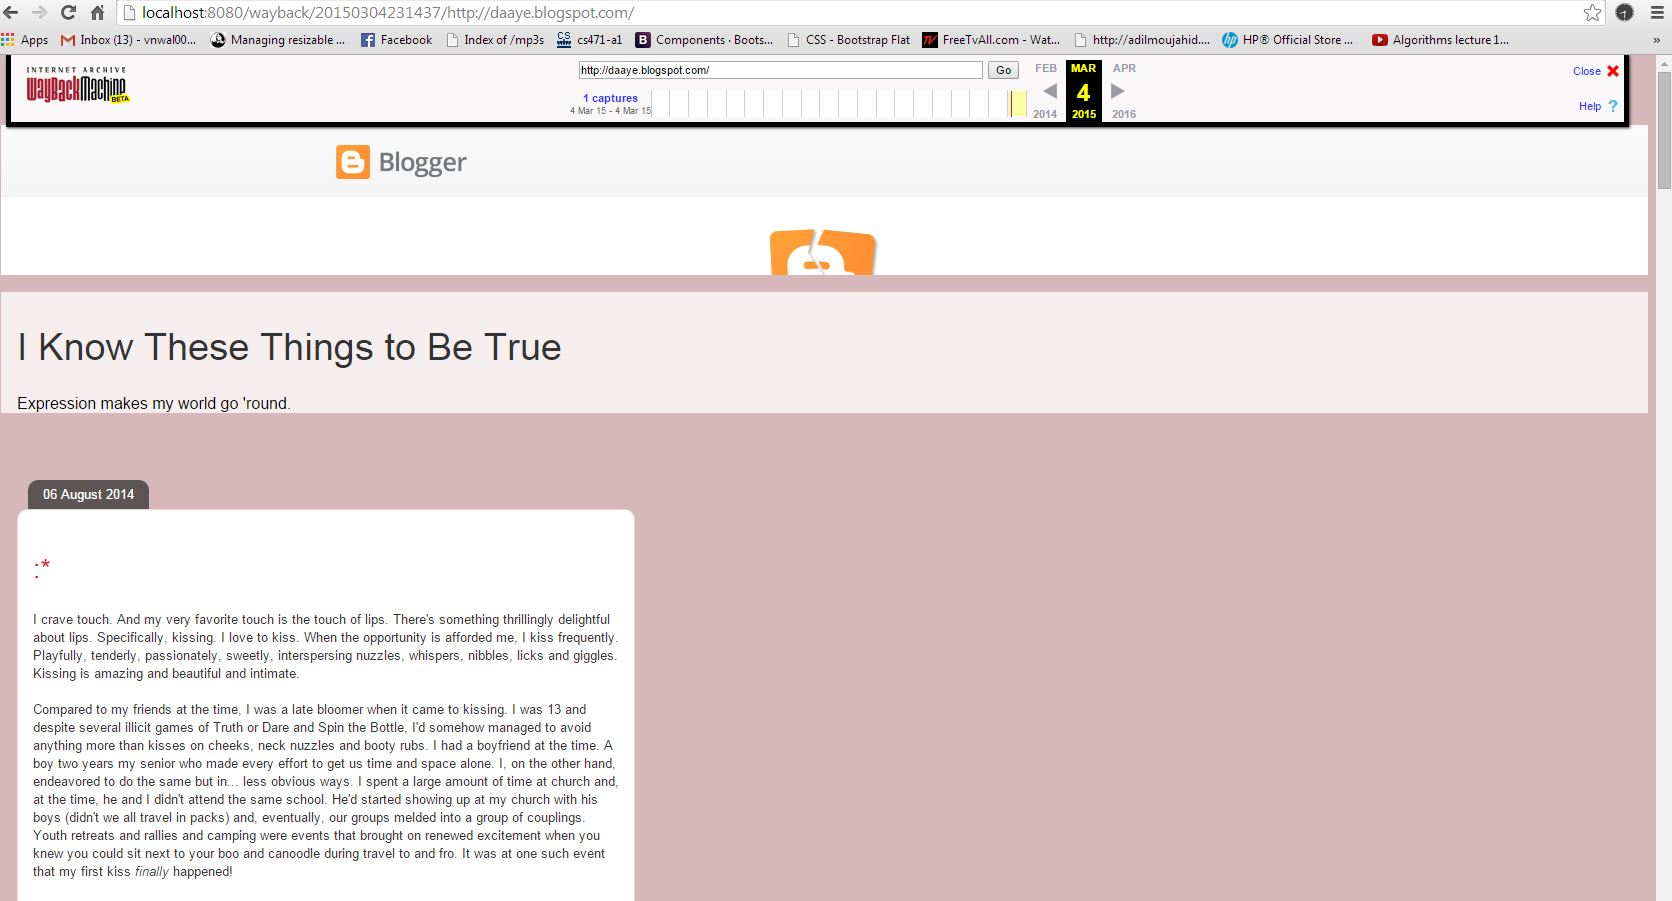
\includegraphics[width=0.75\columnwidth]{SecondWarcReplay} 
\end{center}

I noticed for wayback machine I could only search for 1 URL at a time even if I have a warc file with several URIs, while for webrecorder I could see all URIs in a warc file, then you can click on the link you want. 

\end{homeworkProblem}

%----------------------------------------------------------------------------------------
%	PROBLEM 2
%----------------------------------------------------------------------------------------

\begin{homeworkProblem}

Ingest the 100 URIs from their resulting WARC files into a SOLR instance
see the code + tutorial at: https://github.com/ukwa/webarchive-discovery 
Demonstrate several functioning queries on the files (a full front-end is not required)
describe the configuration choices you made in setting up SOLR and processing the documents.
\newline
The configuration choices I made are still the same as the default settings. Some of which are;
Maximum payload size allowed to be kept wholly in RAM: 10M.
Maximum payload size that will be serialised out to disk instead of held in RAM:100M.
URLs to skip: NONE.
Use the hash+url as the ID for the documents.
Do not check SOLR for duplicates during indexing.
Solr document batch size for submissions: 500.



\begin{center}
{Figure 6: Embedding URIs in SOLR}
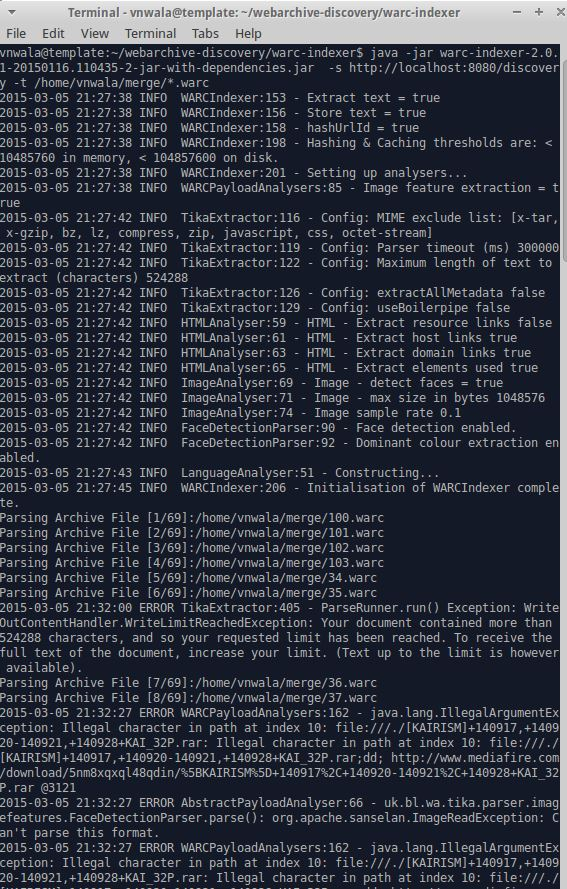
\includegraphics[width=0.75\columnwidth]{solr} 
\end{center}


\begin{center}
{Figure 7: Query for movies}
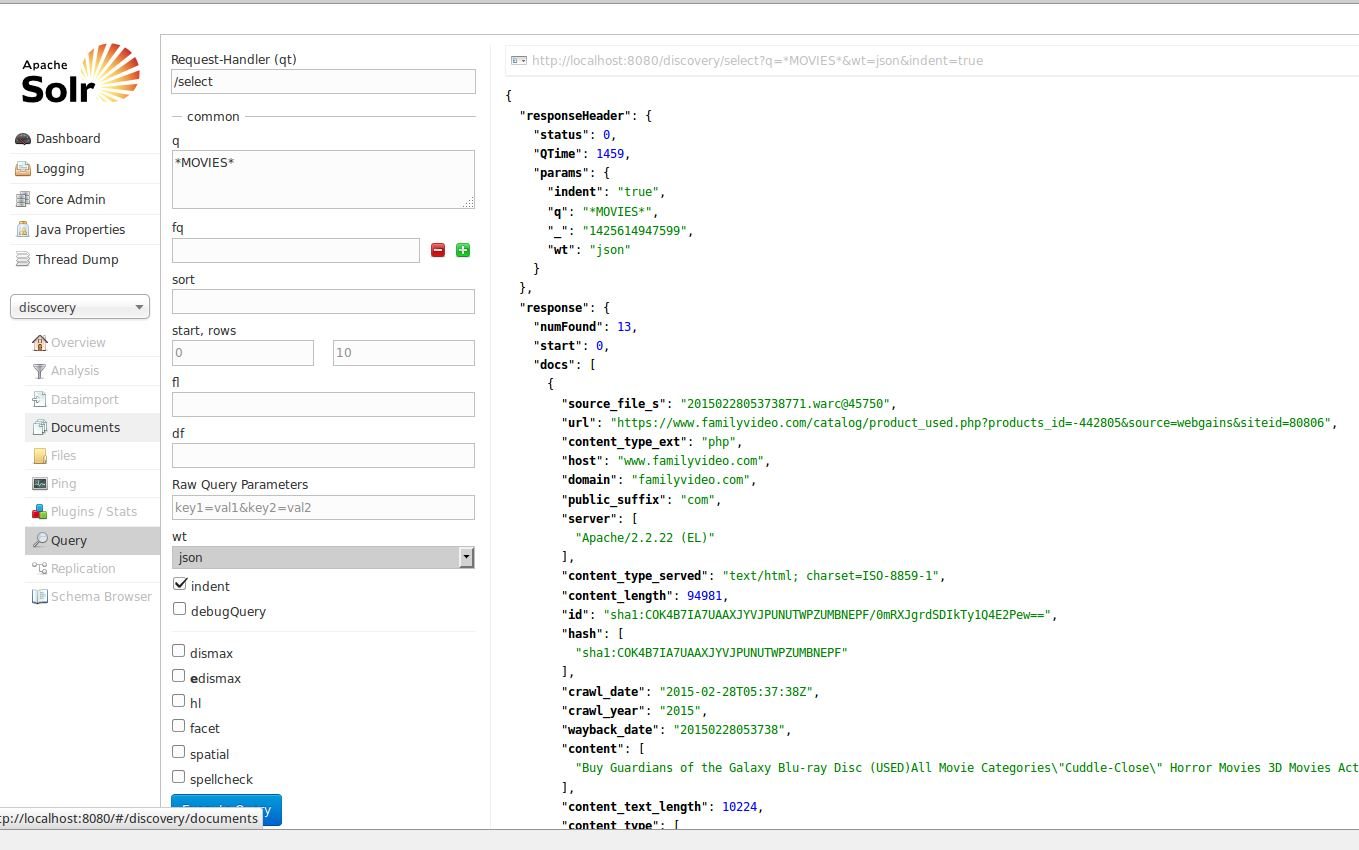
\includegraphics[width=0.75\columnwidth]{movies_query} 
\end{center}

\begin{center}
{Figure 8: Query for domain}
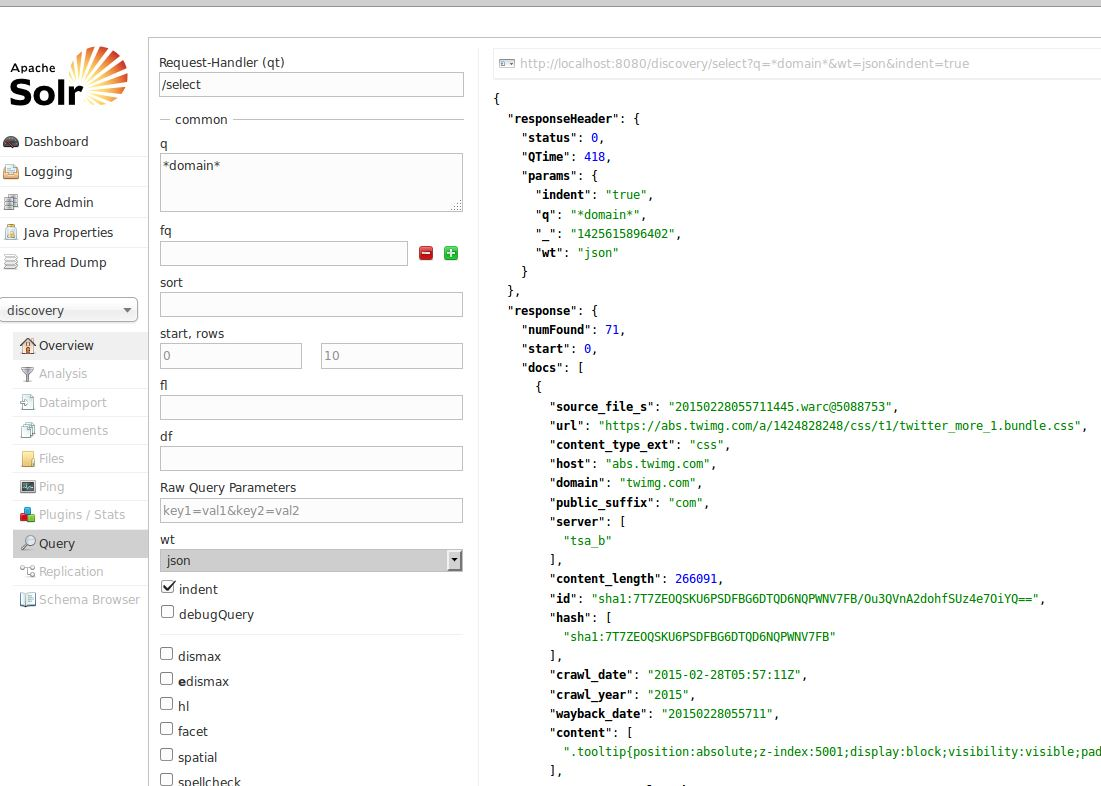
\includegraphics[width=0.75\columnwidth]{domain_query} 
\end{center}

\begin{center}
{Figure 9: Query for files with robot.txt or the word robot, 64 documents with robot.txt files}
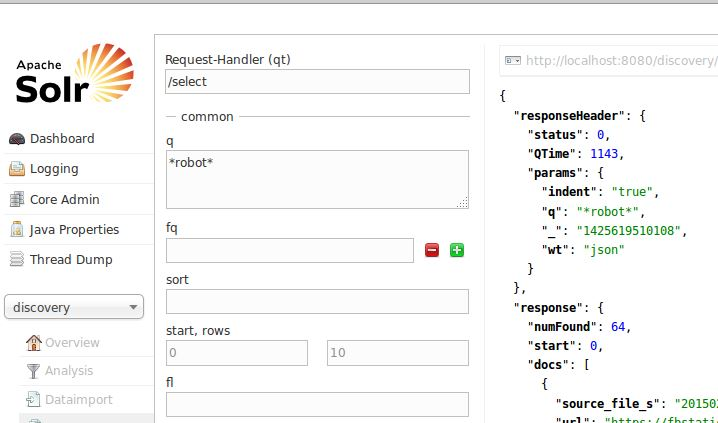
\includegraphics[width=0.75\columnwidth]{robot} 
\end{center}

\section{CONCLUSION}
I could not upload my warc files on github because of their size, I also noticed some URIs did not produce warc files in either Warcreate or Web Recorder. I produced 1 warc file for Heritrix with 100 URIs, while for the rest I did it one at a time and combined them. I am still learning how to query SOLR, hence my querying methods were not really complex. I did not change the configuration of SOLR because I had already uploaded my warc files.



\end{homeworkProblem}

%----------------------------------------------------------------------------------------

\end{document}